\documentclass[]{article}
\usepackage{lmodern}
\usepackage{amssymb,amsmath}
\usepackage{ifxetex,ifluatex}
\usepackage{fixltx2e} % provides \textsubscript
\ifnum 0\ifxetex 1\fi\ifluatex 1\fi=0 % if pdftex
  \usepackage[T1]{fontenc}
  \usepackage[utf8]{inputenc}
\else % if luatex or xelatex
  \ifxetex
    \usepackage{mathspec}
  \else
    \usepackage{fontspec}
  \fi
  \defaultfontfeatures{Ligatures=TeX,Scale=MatchLowercase}
\fi
% use upquote if available, for straight quotes in verbatim environments
\IfFileExists{upquote.sty}{\usepackage{upquote}}{}
% use microtype if available
\IfFileExists{microtype.sty}{%
\usepackage{microtype}
\UseMicrotypeSet[protrusion]{basicmath} % disable protrusion for tt fonts
}{}
\usepackage[margin=1in]{geometry}
\usepackage{hyperref}
\hypersetup{unicode=true,
            pdftitle={Shape of the tuning curve},
            pdfauthor={Rasmus Munter},
            pdfborder={0 0 0},
            breaklinks=true}
\urlstyle{same}  % don't use monospace font for urls
\usepackage{graphicx,grffile}
\makeatletter
\def\maxwidth{\ifdim\Gin@nat@width>\linewidth\linewidth\else\Gin@nat@width\fi}
\def\maxheight{\ifdim\Gin@nat@height>\textheight\textheight\else\Gin@nat@height\fi}
\makeatother
% Scale images if necessary, so that they will not overflow the page
% margins by default, and it is still possible to overwrite the defaults
% using explicit options in \includegraphics[width, height, ...]{}
\setkeys{Gin}{width=\maxwidth,height=\maxheight,keepaspectratio}
\IfFileExists{parskip.sty}{%
\usepackage{parskip}
}{% else
\setlength{\parindent}{0pt}
\setlength{\parskip}{6pt plus 2pt minus 1pt}
}
\setlength{\emergencystretch}{3em}  % prevent overfull lines
\providecommand{\tightlist}{%
  \setlength{\itemsep}{0pt}\setlength{\parskip}{0pt}}
\setcounter{secnumdepth}{0}
% Redefines (sub)paragraphs to behave more like sections
\ifx\paragraph\undefined\else
\let\oldparagraph\paragraph
\renewcommand{\paragraph}[1]{\oldparagraph{#1}\mbox{}}
\fi
\ifx\subparagraph\undefined\else
\let\oldsubparagraph\subparagraph
\renewcommand{\subparagraph}[1]{\oldsubparagraph{#1}\mbox{}}
\fi

%%% Use protect on footnotes to avoid problems with footnotes in titles
\let\rmarkdownfootnote\footnote%
\def\footnote{\protect\rmarkdownfootnote}

%%% Change title format to be more compact
\usepackage{titling}

% Create subtitle command for use in maketitle
\newcommand{\subtitle}[1]{
  \posttitle{
    \begin{center}\large#1\end{center}
    }
}

\setlength{\droptitle}{-2em}
  \title{Shape of the tuning curve}
  \pretitle{\vspace{\droptitle}\centering\huge}
  \posttitle{\par}
  \author{Rasmus Munter}
  \preauthor{\centering\large\emph}
  \postauthor{\par}
  \predate{\centering\large\emph}
  \postdate{\par}
  \date{May 11, 2018}

\usepackage{float}
\usepackage{caption}

\begin{document}
\maketitle

\captionsetup{width=5in}

There are multiple models for how headcells are formed and work. Two of
these are the continous attractor and learning model. The former
predicts that the tuning curve for a HD cell should follow a cosine
curve while the learning model predicts a gaussian tuning curve. To test
these hypotheses the two curves were fit to the tuning curves of the 10
HD cells found in the previous project. The gaussian curve is defined as

\[
f(x) = A + B\cdot\text{exp}\bigg[-\Bigg(\frac{x-P}{C}\bigg)^2\Bigg]
\]

while the cosine curve is defined as

\begin{align*}
    f(x) = 
    \begin{cases}
        A + B \cdot (1 + cos(C\cdot(x-P))) \quad &if\quad |C(x-P)|<\pi \\
        A \quad &else
    \end{cases}
\end{align*}

In our case, \(x\) is the binned head angle and \(f(x)\) is the firing
rate. The capatilized letters are uknown parameters that are tuned by
minimizng the root mean square error between the model and the calculate
tuning curve.

\begin{figure}[H]

{\centering \includegraphics{project2_files/figure-latex/unnamed-chunk-1-1} 

}

\caption{\label{models}\textbf{Models overlaying estimated tuning curve.} A gaussian and cosine curve were fit to the tuning curves by optimizing their tuning parameters to minimize root mean square error. A: Curves for cortex HD cells, B: Curves for thalamus HD cells}\label{fig:unnamed-chunk-1}
\end{figure}

Both models managed to fit a curve relatively well compared to the
actual tuning curve. To compare the two models the RMSE of each model
was plotted in figure \ref{modelRMSE}.

\begin{figure}[H]

{\centering 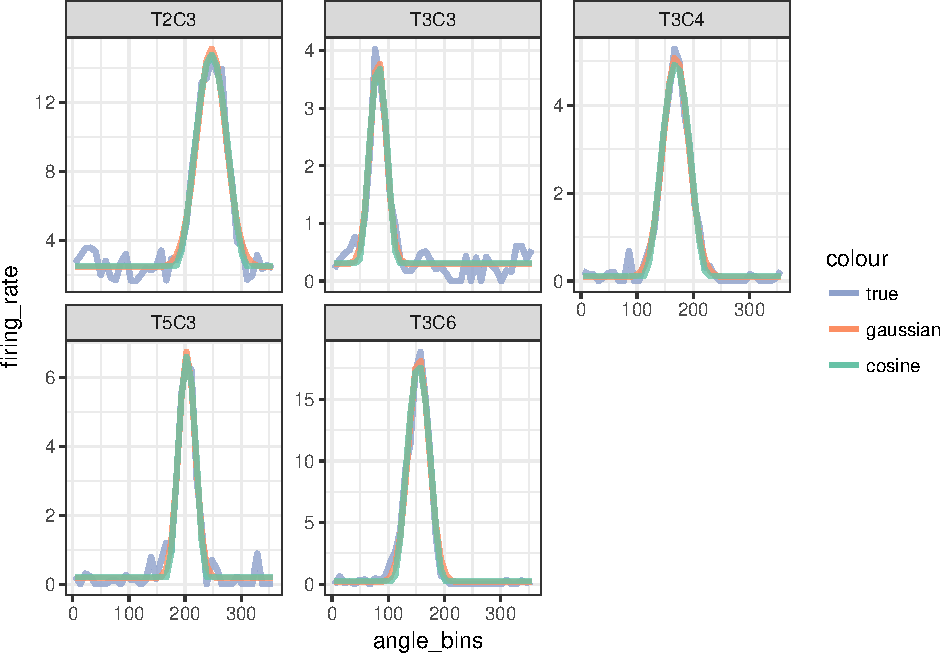
\includegraphics{project2_files/figure-latex/unnamed-chunk-2-1} 

}

\caption{\label{modelRMSE}\textbf{RMSE comparison between models:} The line of best fit indicates that the gaussian curve is a better fit.}\label{fig:unnamed-chunk-2}
\end{figure}

As the gradient of the line of best fit is less than 1 the plot above
suggests that the gaussian curve and thus the learning model is the best
explanation for head direction cells. However since this analysis is
done on only 10 cells and the difference in RMSE is relatively small,
these results are not conclusive.


\end{document}
